\documentclass[a4paper,10pt]{bxjsarticle}
\usepackage[margin=17mm]{geometry}
\usepackage{graphicx}
\usepackage{url}
\title{Kadai Sorter: 課題ファイル整理支援ソフトウェア}
\author{潘東キン（学籍番号：262e140e）}
\date{}
\begin{document}
\maketitle
\vspace{-8mm}

\section{目的と問題点}
大学の授業では、PDF、Pythonファイル、ZIPなど複数形式の課題ファイルを扱う。
現状の問題点は、科目ごとに保存場所が分散し、ファイル名に学籍番号や課題番号を入れ忘れやすいことである。
また、手作業で整理すると、同名ファイルを上書きしたり、提出対象でないファイルを混ぜたりする危険がある。
そこで、課題ファイルを検証してから安全にコピーし、整理結果を監査CSVとして残す
Kadai Sorterを作成した。
リポジトリ：\url{https://github.com/PAN-kobe/kadai-sorter}

\section{実装}
Kadai SorterはPython 3.12で実装したCLIである。
設定ファイルには学籍番号、科目名、科目別名、許可する拡張子を記述する。
プログラムはファイル名をUnicode正規化し、科目、課題番号、学籍番号、拡張子を判定する。
整理計画の作成と実際のコピー処理を分離し、\texttt{scan}ではファイルシステムを変更せずに結果を確認できる。
\texttt{organize}では検証済みファイルだけを出力フォルダにコピーし、既存ファイルや重複する出力先は競合として停止する。
結果はCSVに保存し、\texttt{report}でMatplotlibのグラフを生成する。
品質確認にはpytest、mypy、Ruff、GitHub Actionsを用いた。

\section{有用性の検証}
合成データ500件に対する分類精度は100.0\%、処理時間は11.26ミリ秒であった。
25件、100件、500件の測定では、すべて分類精度100.0\%であり、ファイル数が増えても短時間で処理できた。
単体・統合テストは82件を用意し、学籍番号なし、未対応拡張子、未知の科目、重複出力、既存ファイルなどの失敗ケースを確認した。
特に、同じ出力先になる2件のファイルはどちらもコピーせず、競合として停止することを確認した。

\begin{figure}[h]
\centering
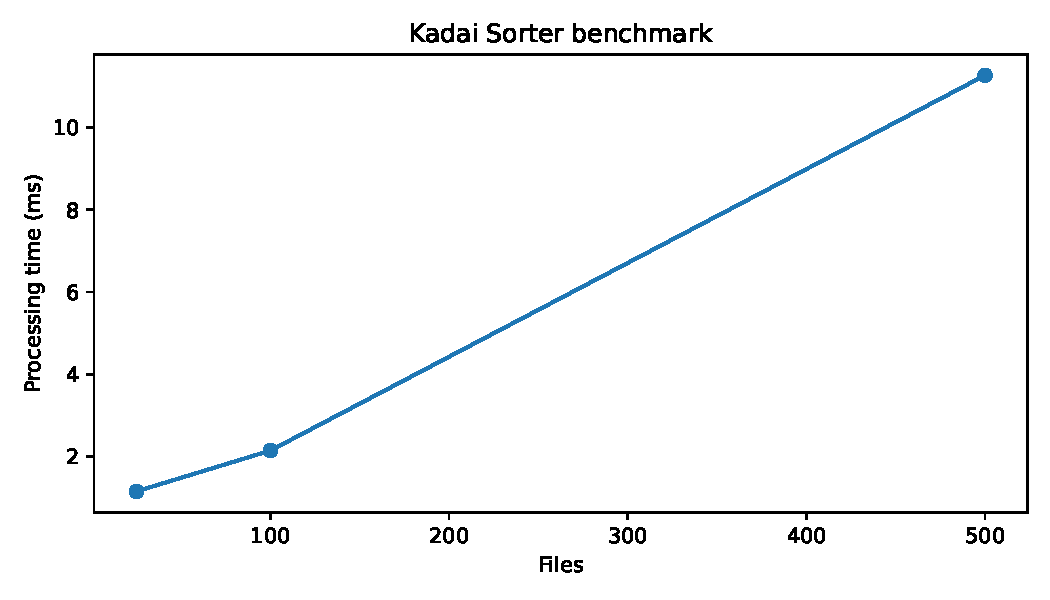
\includegraphics[width=.72\linewidth]{benchmark.pdf}
\caption{ファイル数と処理時間}
\end{figure}

\section{AIの使用}
OpenAI Codexを、課題要件の整理、設計案、実装補助、テストケース作成、READMEとレポート文面の作成、最終確認に使用した。
ただし、測定値は生成結果を推測せず、実際に作成した\texttt{benchmark.csv}とテスト結果を確認して記載した。

\end{document}
